% yaml_bridge.tex
% Simple, clean diagram for Stata Journal
% Shows YAML as a bridge between Stata and modern data science ecosystem
% Author: João Pedro Azevedo
% Date: December 2025

\documentclass[tikz,border=8pt]{standalone}
\usepackage{tikz}
\usetikzlibrary{positioning, arrows.meta, calc}

\begin{document}

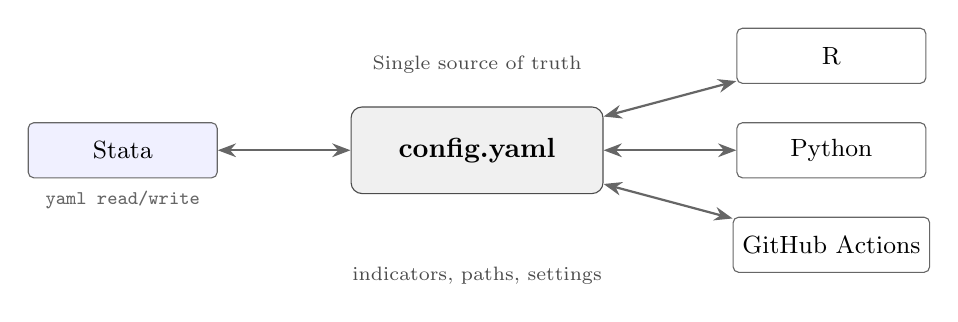
\begin{tikzpicture}[
    % Clean, minimal styles
    toolbox/.style={
        rectangle, 
        rounded corners=2pt,
        draw=black!60, 
        fill=white,
        minimum width=2.4cm, 
        minimum height=0.7cm,
        font=\small
    },
    yamlbox/.style={
        rectangle, 
        rounded corners=4pt,
        draw=black!70, 
        fill=gray!12,
        minimum width=3.2cm, 
        minimum height=1.1cm,
        font=\normalsize\bfseries
    },
    arrow/.style={
        <->,
        >=Stealth,
        thick,
        black!60
    },
    labelstyle/.style={
        font=\scriptsize,
        text=black!70
    }
]

% === Central: YAML Configuration ===
\node[yamlbox] (yaml) at (0, 0) {config.yaml};

% === Left: Stata with yaml command ===
\node[toolbox, fill=blue!6] (stata) at (-4.5, 0) {Stata};
\node[font=\scriptsize\ttfamily, below=1pt of stata, text=black!60] {\texttt{yaml read/write}};

% === Right column: Other tools ===
\node[toolbox] (r) at (4.5, 1.2) {R};
\node[toolbox] (python) at (4.5, 0) {Python};
\node[toolbox] (github) at (4.5, -1.2) {GitHub Actions};

% === Arrows ===
\draw[arrow] (stata) -- (yaml);
\draw[arrow] (yaml) -- (r);
\draw[arrow] (yaml) -- (python);
\draw[arrow] (yaml) -- (github);

% === Labels ===
\node[labelstyle, above=0.3cm of yaml] {Single source of truth};
\node[labelstyle, below=0.8cm of yaml] {indicators, paths, settings};

\end{tikzpicture}

\end{document}
